\documentclass{extarticle}
\usepackage[left=2cm,right=1.5cm,top=1.5cm, bottom=1.5cm]{geometry}

\usepackage{multirow}
\usepackage{hyperref}
\usepackage{url}

\usepackage{graphicx}
\usepackage{wrapfig}

\usepackage[utf8]{inputenc}
\usepackage[T1]{fontenc}
\usepackage[english, russian]{babel}

\usepackage{float}


\begin{document}

\begin{titlepage}
	\begin{center}
		
		
		\textsc{\textbf{пояснительная записка \\
				к выпускной квалификационной работе на тему}}\\[2cm]
		
		% Title
		\textsc{Исследование влияния возможных систематических ошибок на результаты эксперимента по изучению временной инваринтности на ускорителе COSY \\[2.4cm] }
		
		
	\end{center}
	
	
	\begin{flushright}
		% Author and supervisor
		\begin{tabular}{rr}
			Студент-дипломник \underline{\hspace*{3cm}} & А.Е. Аксентьев \\
			&	группа А12-06 \\					
			Научный руководитель: Dr. rer. nat. \underline{\hspace*{3cm}} & Ю.В. Вальдау \\
			Консультант:          Доц., к.ф.-м.н. \underline{\hspace*{3cm}} & С.М. Полозов 	\\
			Рецензент:			  Доц., к.ф-м.н. \underline{\hspace*{3cm}} & А.А. Тищенко \\
			Зав. кафедрой:		  Проф., д.ф.-м.н. \underline{\hspace*{3cm}} & А.Н. Диденко
		\end{tabular}
		
	\end{flushright}
	
	\vfill
	
	
	\begin{center}
		\the\year{}
	\end{center}
	
	
	
\end{titlepage}

\tableofcontents
\pagebreak

\section*{Введение}
JEDI-коллаборация (J\"ulich Electric Dipole Moment Investigations) была создана в 2011 году с целью провести долгосрочный проект по измерению электрического дипольного момента (ЭДМ) заряженных частиц в накопительном кольце (srEDM: Storage Ring EDM). На текущий момент, коллаборация базируется на синхротроне COSY (Institut f\"ur Kernphysik, Forschungszentrum J\"ulich, Юлих, Германия), где разрабатывает концептуальный дизайн накопительного кольца для поиска дейтронного ЭДМ.

Поиск Электрического Дипольного Момента (ЭДМ) в невырожденных системах был инициирован Эдвардом Пёрселлом и Норманом Рэмзи более 50 лет назад, для нейтрона. С тех пор было проведено множество всё более чувствительных экспериментов на нейтронах, атомах, и молекулах, и тем не менее, ЭДМ пока ещё не был обнаружен. 

Интерес поиска ЭДМ в том, что, если они существуют, они нарушают P- и T-симметрии. Дело в том, что вся наблюдаемая вселенная состоит преимущественно из материи; антиматерия может быть получена в ускорителях заряженных частиц, но в пренебрежимо малых количествах. На сколько мы понимаем, вскоре после Большого Взрыва, материя была образована из энергии в парах частица-античастица, после чего последовала стадия аннигиляции --- превращения пары частица-античастица обратно в энергию, --- однако по какой-то причине, эта фаза закончилась превалированием материи над антиматерией (по крайней мере в наблюдаемой вселенной) --- процесс называемый \emph{бариогенезом.}

В 1967 году, академик АН СССР Андрей Сахаров определил условия, требуемые для бариогенеза (независимо от механизма его действия). Одно из \emph{условий Сахарова} --- существование процессов, нарушающих C- и CP-симметрии. Известны источники нарушения этих симметрий, однако их не достаточно для объяснения барионной асимметрии вселенной; поиск продолжается.

Ненулевые ЭДМ элементарных частиц могут привести нас к физике за границами Стандартной Модели элементарных частиц; такие теории как SUSY (суперсимметрия) указывают на наличие ЭДМ гораздо больше, чем предсказывает Стандартная Модель элементарных частиц.

Проект srEDM --- это сложное, high-risk high-impact предприятие, нуждающееся в тщательном планировании и исполнении. Далее описаны структура требуемой команды экспертов, оборудования, и ступени развития проекта.

\section{Структура команды и партнёры}
Несмотря на то, что Институт ядерной физики исследовательского центра ``Юлих'' (IKP FZ J\"ulich) --- включающий в себя отдел ускорителей, а также центральные инженерные институт (ZEA, специализирующиеся в механике и электронике), --- предоставляет крепкий фундамент для предложенного проекта srEDM, многогранность и сложность проекта требуют  дополнительной экспертизы, предоставляемой следующими институтами:
\begin{itemize}
	\item Институт физики Рейн-Вестфальского Технического Университета (RWTH) Аахена обладает международно-признанными экспертами в области дизайна и конструкции компонент детекторов, а также анализа данных; этот аспект крайне важен в разработке требуемого для эксперимента поляриметра. Профессор этого института Йорг Претц участвовал в коллаборации $(g-2)_{\mu}$ Брукхейвенской Национальной Лаборатории (BNL), единственном до сих пор прецезионном эксперименте в накопительном кольце.
	\item Исследовательская группа Университета Феррары и INFN (UNIFE) под предводительством профессора Паоло Ленисы давно сотрудничает с IKP FZJ в таких экспериментах как PAX (Proton-Antiproton eXperiment), и приобрела уникальную экспертизу в области поляризованных источников, мишеней, и поляриметрии, что является чрезвычайно ценным для успеха поляриметрии во всех экспериментах COSY.
\end{itemize}

Также, FZJ и RWTH основали институт JARA (J\"ulich-Aachen Research Alliance), с группой FAME (Forces and Matter Experiments), с целью изучения вопроса о судьбе антиматерии. JARA-FAME включаетс все институты FZJ и RTWH; вместе UNIFE и JARA-FAME составляют коллаборацию JEDI. На сегодняшний день, коллаборация включает в себя 132 члена.

\begin{figure}[H]
	\centering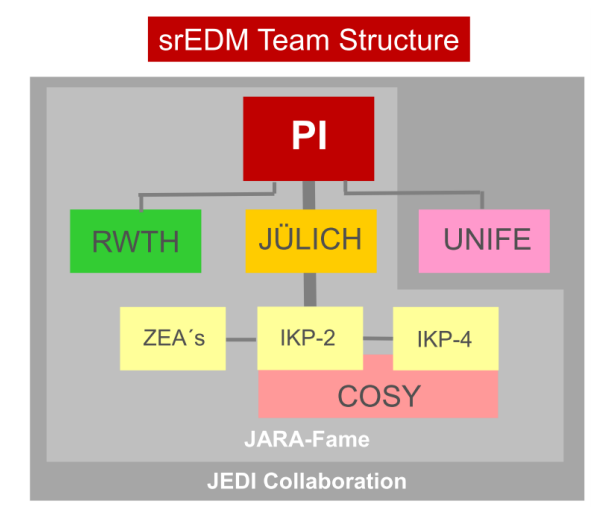
\includegraphics[scale=.7]{img/JEDI_architecture}
\end{figure}

\section{Финансирование}
Финансирование проекта производится засчёт гранта srEDM Европейского Совета по Научным Исследованиям (European Research Council). Бюджет проекта составляет в целом  2,467,713 евро; из них 47\% уйдут в FJZ, 28\% в RWTH Aachen, и оставшиеся 25\% в UNIFE. Смета проекта srEDM представлена в следующей таблице:

\begin{figure}[H]
	\centering
	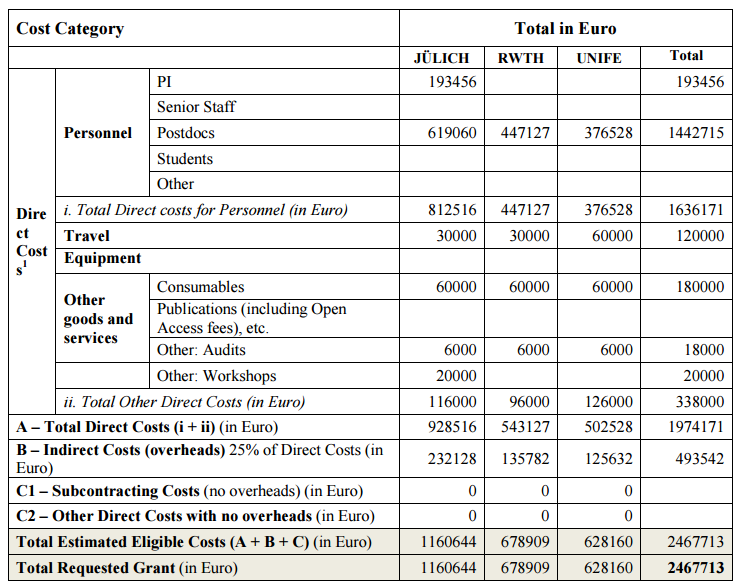
\includegraphics[scale=.7]{img/Costs_Table}
\end{figure}

\section{Контроль производства}
Для обеспечения успешности проекта, вся работа разделена на несколько пакетов (work packages) производимых результатов. Все результаты попадают под одну из двух категорий: Ключевые технологии, и Измерения в накопительном кольце.

\begin{figure}[H]
	\centering
	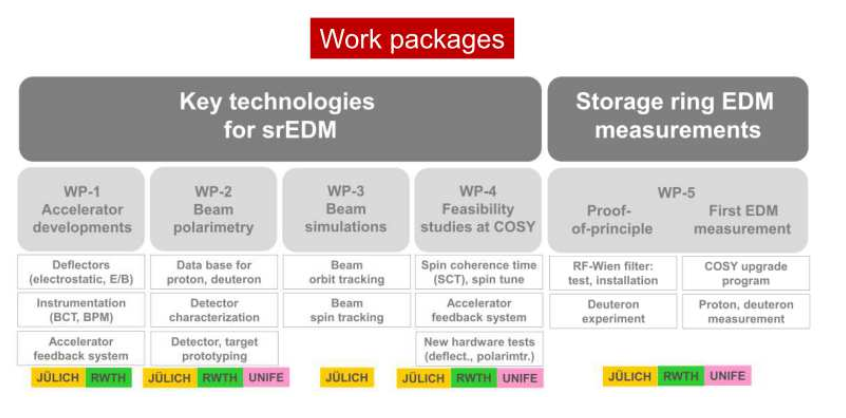
\includegraphics[scale=.5]{img/Work_packages}
\end{figure}
		
\section*{Заключение}
На данный момент, в исследовательской программе CERN планируется пауза на десять лет. В связи с этим рассматривается список задач фундаментальной физики, которыми можно было бы заняться в это время. Среди приоритетных задач этого списка --- поиск ЭДМ. 

Поскольку протонное кольцо можно сделать полностью электростатическим (позволяет величина $G$), в то время как дейтронное принципиально требует магнитные элементы, если ЦЕРН решит заняться поиском ЭДМ, вероятнее всего будет построено протонное кольцо.
\begin{thebibliography}{0}
	\bibitem{JEDIatJuelich}
	Institute for Nuclear Physics, IKP-2: Experimental Hadron Dynamics. \url{http://www.fz-juelich.de/ikp/ikp-2/EN/Forschung/JEDI/_node.html}
	\bibitem{ERCGrant10}
	Str\"oher, H. Пресс-конференция. \url{https://www.fz-juelich.de/SharedDocs/Videos/PORTAL/EN/erc/erc-grant-stroeher.html}
	\bibitem{ERCGrant16}
	Lenisa, P., Pretz, J., Str\"oher, H. (2016). Storage ring steps up search for electric dipole moments. \textit{CERN Courier}. \url{http://cerncourier.com/cws/article/cern/65816}
	\bibitem{ERCGrant12}
	Rathmann, F. Application for an ERC Advanced Grant 2012. \url{http://collaborations.fz-juelich.de/ikp/jedi/public_files/proposals/merged_document.pdf}
	\bibitem{ERCGrant15}
	Str\"oher, H., Search for Electric Dipole Moments using Storage Rings, Horizon 2020 proposal, Excellence Science Call: ERC-2015-AdG. \url{http://collaborations.fz-juelich.de/ikp/jedi/public_files/proposals/Proposal-SEP-210276270.pdf}
	\bibitem{JEDI}
	JEDI Collaboration. \url{http://collaborations.fz-juelich.de/ikp/jedi/index.shtml}
	\bibitem{BNL}
	D. Anastassopoulos, V. Anastassopoulos, D. Babusci. AGS Proposal: Search for a permanent electric dipole moment of the deuteron nucleus at the $10^{-29} e\cdot cm$ level. [Internet]. BNL; 2008 [cited 2016 Nov 25]. Available from: \url{https://www.bnl.gov/edm/files/pdf/deuteron_proposal_080423_final.pdf}
	\bibitem{Senichev}
	Yurij Senichev. Search for the Charged Particle Electric Dipole Moments in Storage Rings. In: 25th Russian Particle Accelerator Conf(RuPAC’16), St Petersburg, Russia, November 21-25, 2016 [Internet]. JACOW, Geneva, Switzerland; 2017 [cited 2017 Apr 5]. p. 6–10. Available from: \url{http://accelconf.web.cern.ch/AccelConf/rupac2016/papers/mozmh03.pdf}
	
\end{thebibliography}
\end{document}